\documentclass[9pt]{beamer}
\mode<presentation>

% Theme choice:
\usetheme{Madrid}%Darmstadt 

\usecolortheme[RGB={0,100,50}]{structure}
 \usefonttheme{structurebold} 
\setbeamercovered{invisible}
%\setbeamertemplate{navigation symbols}{}
\usepackage{dynblocks}
\usepackage{textpos}
\usepackage{amsfonts}
\usepackage{amsmath}
\usepackage{amssymb}
\usepackage{amsthm}
\usepackage{mathtools}
\usepackage{dutchcal}
\usepackage{hyperref}
\usepackage[utf8]{inputenc}
\usepackage[T1]{fontenc}
% Title page details: 
\title[Beamer Name]{Assignment 5 - Smart Contracts} %add title


\author[N. K. Muga]{ \textbf{\Large Naveen Kumar Muga}} %Add author
\institute[UAB]{\large nmuga@uab.edu} 
%\titlegraphic{\includegraphics[width=5cm]{Logo1.eps}}
\date{}

% Logo only on title page
%\logo{\includegraphics[width=1cm,keepaspectratio]{Logo.png}}
\usepackage[pscoord]{eso-pic}


\begin{document}

% Title page frame
%\begin{frame}
    %\titlepage 
%\end{frame}
\frame[plain]{\titlepage}
%logo
\AddToShipoutPictureFG{
    \put(\LenToUnit{.92\paperwidth},
    \LenToUnit{.185\paperheight})
    {\vtop{{\null}
    \makebox{
\includegraphics[width=.8cm,keepaspectratio]{public/blockchain.png}}}}}


\begin{frame}{Outline}
  \tableofcontents
\end{frame}

\section{Overview}

\begin{frame}{Project idea}
    The project goal is to build complete distributed marketplace based on ethereum using following technologies:
    \begin{description}
        \item[Node.js] an open-source, cross-platform JavaScript runtime environment,
        \item[React.js] a free and open-source front-end JavaScript library for building user interfaces based on UI components,
        \item[Ethereum] is a decentralized, open-source blockchain with smart contract functionality,
        \item[IPFS] a protocol, hypermedia and file sharing peer-to-peer network for storing and sharing data in a distributed file system
        \item[Solidity] is an object-oriented programming language for implementing smart contracts on various blockchain platforms, most notably, Ethereum,
        \item[Web3.js] is a collection of libraries that allow you to interact with a local or remote ethereum node using HTTP, IPC or WebSocket;
    \end{description}
\end{frame}

\begin{frame}{Technologies Overview}
    While Node.js and React.js are just platform for running os independent JavaScript code and building user interface, let's focus on IPFS, Solidity, Ethereum and Web3.js.
\end{frame}

\begin{frame}{Ethereum}
    Ethereum allows anyone to deploy permanent and immutable decentralized applications onto it, with which users can interact. Decentralized finance (DeFi) applications provide a broad array of financial services without the need for typical financial intermediaries like brokerages, exchanges, or banks, such as allowing cryptocurrency users to borrow against their holdings or lend them out for interest. Ethereum also allows users to create and exchange NFTs, which are unique tokens representing ownership of an associated asset or privilege, as recognized by any number of institutions.
    
    Support for Smart Contracts which enables developers to build state machines and store some limited data over blockchain. Why limited? Because storing data in blockchain requires payment. According to the yellow paper, the fee is 20k gas to store a 256 bit word. A kilobyte is thus 640k gas. To beat this some decentralized storage must be used. 
\end{frame}

\begin{frame}{IPFS}
    The Interplanetary File System (IPFS) is a decentralized file system for building the next generation of the internet. Filecoin (opens new window) and many popular Web3 projects are built on IPFS. Some call it the hard drive for blockchain and Web3, though its power extends much further. This distributed hash based filesystem enables developers to store data like images or product description in decentralized manner. 
    
    Merging this technology with blockchain Smart Contracts allows to store fg. product description as JSON document in IPFS and reference to it in Smart Contract. Which is effective solution.
\end{frame}

\begin{frame}{Solidity}
    Solidity is an object-oriented, high-level language for implementing smart contracts. Smart contracts are programs which govern the behaviour of accounts within the Ethereum state. Solidity is a curly-bracket language designed to target the Ethereum Virtual Machine (EVM). It is influenced by C++, Python and JavaScript.
    
    Which allows developers to write small program in high level language that address ethereum virtual machine.
\end{frame}

\begin{frame}{Web3.js}
    Web3 is a collection of JS libraries that lets you interact with an Ethereum node remotely or locally. Simply, it provides us with an API to use so we can easily work with the blockchain. Web3 works as a wrapper for JSON RPC to connect to a remote or local Ethereum node with either a HTTP or IPC connection.
    
    This is a heart of an application that allows interacting with ethereum blockchain for storing, manipulating and retrieving smart contracts data.
\end{frame}

\section{Architecture and Design}

\begin{frame}{Architecture Overview}
   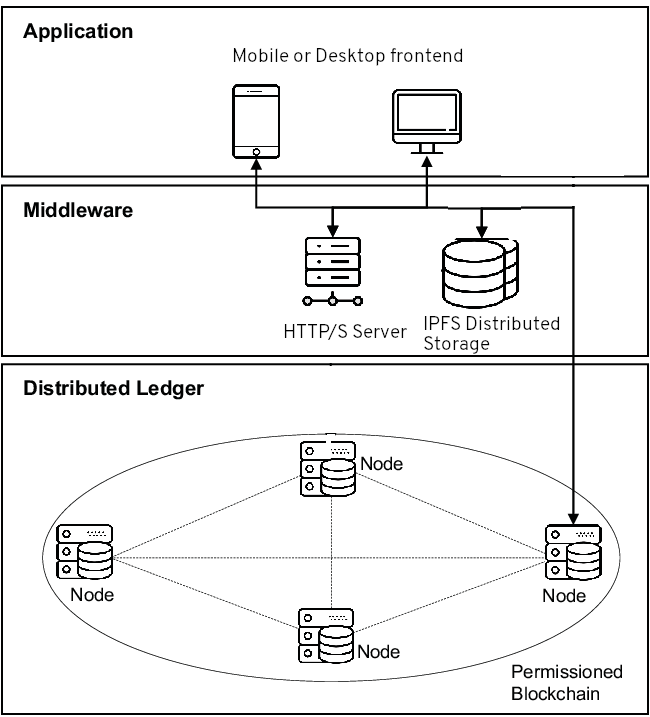
\includegraphics{arch}
\end{frame}

\begin{frame}{Description}
   Application runs in a blockchain enabled web browser using bundled JavaScript libraries, HTTPS/S web server is needed for distributing the application files are stored using IPFS distributed storage. Operations on smart contracts are handled by ethereum network.
\end{frame}

\begin{frame}{Frame 2.2}

\end{frame}

\section{Limitations}
    \begin{frame}{Improvements}
        \begin{itemize}
            \item No sellers reputation, some way of storing it must be figured out while keeping application opensource 
            \item Currently no way of sending questions about product to seller
            \item The worst no escrow service funds are transferred to seller before sending product digital or physical this may lead to scams
        \end{itemize}
    \end{frame}
\section{Lessons learned}
    \begin{frame}{Knowledge}
        \begin{itemize}
            \item Selling physical or digital goods over decentralized marketplace needs 3rd party adversary acting like escrow service, this can be done by implementing multisignature transactions. 
            
            \item Storing data over blockchain is not cost effective some other technologies must be used to build fully decentralized marketplace with products images and descriptions.
        \end{itemize}
    \end{frame}
\end{document}
